\documentclass[aspectratio=169,11pt]{beamer}
\usetheme{Madrid}
\usecolortheme{default}

\usepackage{amsmath,amssymb}
\usepackage{booktabs}
\usepackage{graphicx}
\usepackage{hyperref}

\title{Presentation II: Research / Contribution}
\subtitle{DiT + Diffusion Forcing for Interactive Billiards Physics}
\author{Your Name}
\date{\today}

\begin{document}

\begin{frame}
  \titlepage
\end{frame}

\begin{frame}{Agenda}
\begin{enumerate}
  \item Research question and novelty
  \item What we built (data \(\rightarrow\) VAE \(\rightarrow\) world model \(\rightarrow\) interactive inference)
  \item Quantitative findings (historical and near-fair reruns)
  \item Qualitative findings + failure modes
  \item Hardships/debugging journey
  \item Final takeaways and next steps
\end{enumerate}
\end{frame}

\begin{frame}{Research Question and Hypothesis}
\textbf{Research question:}
\begin{quote}
Can diffusion forcing help an action-conditioned DiT preserve interactive billiards physics better than baseline single-step training?
\end{quote}
\vspace{0.4em}
\textbf{Hypothesis:}
\begin{itemize}
  \item DF should improve long-horizon rollouts by training on partially self-generated context.
  \item Expected gains: collision continuity and wall-bounce stability.
  \item Remaining risk: identity consistency (color drift/swallowing artifacts).
\end{itemize}
\end{frame}

\begin{frame}{What Is Novel Here?}
\begin{itemize}
  \item Focus on \textbf{interactive physics consistency}, not only image quality.
  \item Controlled multi-dataset strategy (v1/v2/v3) to stress different behaviors.
  \item Direct baseline-vs-DF rollout comparisons with fixed horizons.
  \item Explicit failure analysis: collision validity vs identity consistency.
\end{itemize}
\end{frame}

\begin{frame}{Project Journey (What We Actually Did)}
\begin{itemize}
  \item Built large simulation pipeline and collected staged datasets (v1/v2/v3).
  \item Trained VAE and exported latent shards for scalable world-model training.
  \item Trained DiT baselines, then implemented and trained Diffusion Forcing (DF).
  \item Scaled to larger runs (joint datasets, up to \(\sim\)1.52B model line).
  \item Built interactive inference/UI routes and tested action-conditioned behavior.
\end{itemize}
\vspace{0.4em}
\textbf{Main scientific thread:} does DF preserve rollout physics better?
\end{frame}

\begin{frame}{Dataset Strategy (v1/v2/v3)}
\begin{table}
\centering
\begin{tabular}{lccp{4.2cm}}
\toprule
Dataset & Episodes & Frames/ep & Purpose \\
\midrule
v1 & 100k & 600 & Baseline coverage \\
v2 & 100k & 600 & More diversity/randomization \\
v3 & 200k & 600 & Collision-heavy hard cases \\
\bottomrule
\end{tabular}
\end{table}
\vspace{0.2em}
This staged design improved robustness and made collision behavior easier to learn.
\end{frame}

\begin{frame}{World Model Setup We Compared}
\begin{itemize}
  \item Same backbone family for key baseline/DF comparisons:
  \begin{itemize}
    \item \(d_{\text{model}}=768\), 10 layers, 12 heads, context length \(L=8\)
  \end{itemize}
  \item Baseline objective: single-step diffusion noise prediction
  \item DF objective: rollout training with context updates under scheduled teacher forcing
  \item Rollout eval: horizons \(h=\{1,4,8,16,32\}\), DDIM=10, same VAE decoder
\end{itemize}
\end{frame}

\begin{frame}{Experimental Setup (Main Comparison)}
\textbf{Historical comparison (reported earlier):}
\begin{itemize}
  \item Baseline: \(60\)M samples
  \item DF: \(120\)M total samples
\end{itemize}
\vspace{0.4em}
\textbf{Near-fair check (run now):}
\begin{itemize}
  \item Baseline exact: \(60.0\)M checkpoint
  \item DF smoke: \(60.2\)M checkpoint (resume + 200k with DF)
  \item Same eval pipeline, same horizons, same DDIM steps
\end{itemize}
\end{frame}

\begin{frame}{Historical Result (60M Baseline vs 120M DF)}
\begin{table}
\centering
\begin{tabular}{lcccc}
\toprule
Model & MSE@16 & MSE@32 & PSNR@16 & PSNR@32 \\
\midrule
Baseline 60M & 54.023 & 318.312 & 17.133 & 14.857 \\
DF 120M & 0.763 & 0.827 & 19.447 & 19.372 \\
\bottomrule
\end{tabular}
\end{table}
\vspace{0.3em}
\textbf{Caveat:} this is strong but not a strict apples-to-apples budget comparison.
\end{frame}

\begin{frame}{Key Result Table (Near-Fair 60.0M vs 60.2M)}
\begin{table}
\centering
\begin{tabular}{lcccc}
\toprule
Model & MSE@16 & MSE@32 & PSNR@16 & PSNR@32 \\
\midrule
Baseline 60.0M & 54.023 & 318.312 & 17.133 & 14.857 \\
DF 60.2M & 1.238 & 1.597 & 18.809 & 18.063 \\
\bottomrule
\end{tabular}
\end{table}
\vspace{0.4em}
\footnotesize
Source: \texttt{rollout\_eval\_ctx8\_baseline60m\_vs\_df60p2m\_20260303}
\end{frame}

\begin{frame}{Sanity Check (Different Eval Seed)}
\begin{itemize}
  \item Repeated eval with a different seed (different sampled clips).
  \item Pattern stayed the same:
  \begin{itemize}
    \item Baseline MSE@16/32 remained very high.
    \item DF MSE@16/32 remained low.
  \end{itemize}
\end{itemize}
\begin{table}
\centering
\begin{tabular}{lcc}
\toprule
Metric & Baseline (seed123) & DF (seed123) \\
\midrule
MSE@16 & 105.241 & 1.268 \\
MSE@32 & 414.579 & 1.378 \\
\bottomrule
\end{tabular}
\end{table}
\end{frame}

\begin{frame}{Control Check: Is It Just +200k Training Steps?}
\begin{itemize}
  \item We ran a baseline control from 60.0M \(\rightarrow\) 60.2M (no DF) with matched resume-smoke style.
  \item Result: baseline control got worse at long horizon.
\end{itemize}
\begin{table}
\centering
\begin{tabular}{lcc}
\toprule
Model & MSE@16 & MSE@32 \\
\midrule
Baseline 60.0M & 54.0 & 318.3 \\
Baseline control 60.2M & 2022.5 & 5379.9 \\
DF 60.2M & 1.289 & 1.766 \\
\bottomrule
\end{tabular}
\end{table}
\end{frame}

\begin{frame}{Interpretation: Why This Big Gap Can Happen}
\begin{itemize}
  \item Inference is autoregressive: model consumes its own predicted context.
  \item One-step baseline is underexposed to this regime during training.
  \item DF explicitly trains multi-step context replacement:
\[
\tilde z_{k+1}=m_k z_{k+1}^{gt}+(1-m_k)\hat x_{0,k}
\]
  \item This reduces train/inference mismatch and mitigates long-horizon error explosion.
\end{itemize}
\end{frame}

\begin{frame}{Qualitative Findings}
\begin{columns}[T]
\column{0.48\textwidth}
\textbf{What works better}
\begin{itemize}
  \item wall bounces generally correct
  \item collisions more coherent
  \item less long-horizon drift
\end{itemize}
\column{0.48\textwidth}
\textbf{What still fails}
\begin{itemize}
  \item color identity drift
  \item occasional swallowing/merging
  \item interactive latency still high
\end{itemize}
\end{columns}
\vspace{0.4em}
\centering
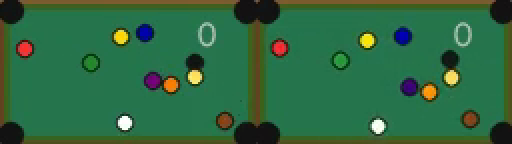
\includegraphics[width=0.64\linewidth]{../final_project_essay/assets/latest_resume555m_clip_002.png}
\end{frame}

\begin{frame}{Scaling Findings (Beyond Baseline vs DF)}
\begin{itemize}
  \item As we scaled data/model, short-to-mid horizon quality generally improved.
  \item Gains were not strictly monotonic for every horizon/metric.
  \item Practical takeaway:
  \begin{itemize}
    \item scaling helps,
    \item but training regime and rollout robustness matter just as much.
  \end{itemize}
\end{itemize}
\end{frame}

\begin{frame}{Metric Trend Visuals}
\begin{columns}[T]
\column{0.5\textwidth}
\centering
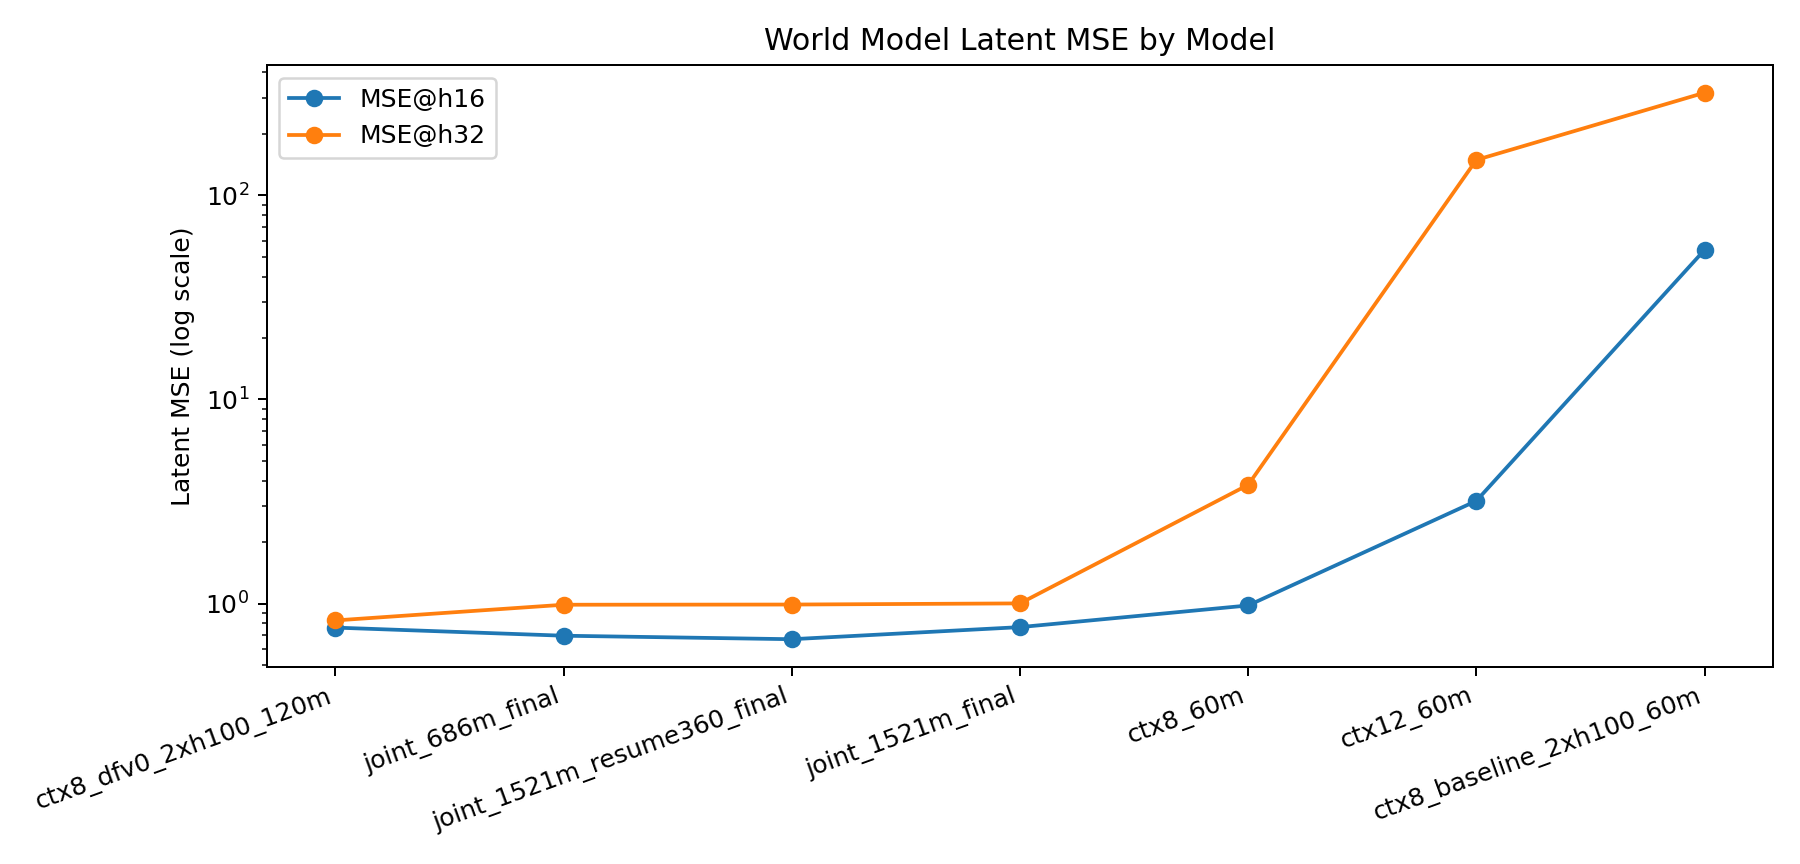
\includegraphics[width=\linewidth]{../../milestones_preview/charts/world_model_mse_h16_h32_log.png}
\column{0.5\textwidth}
\centering
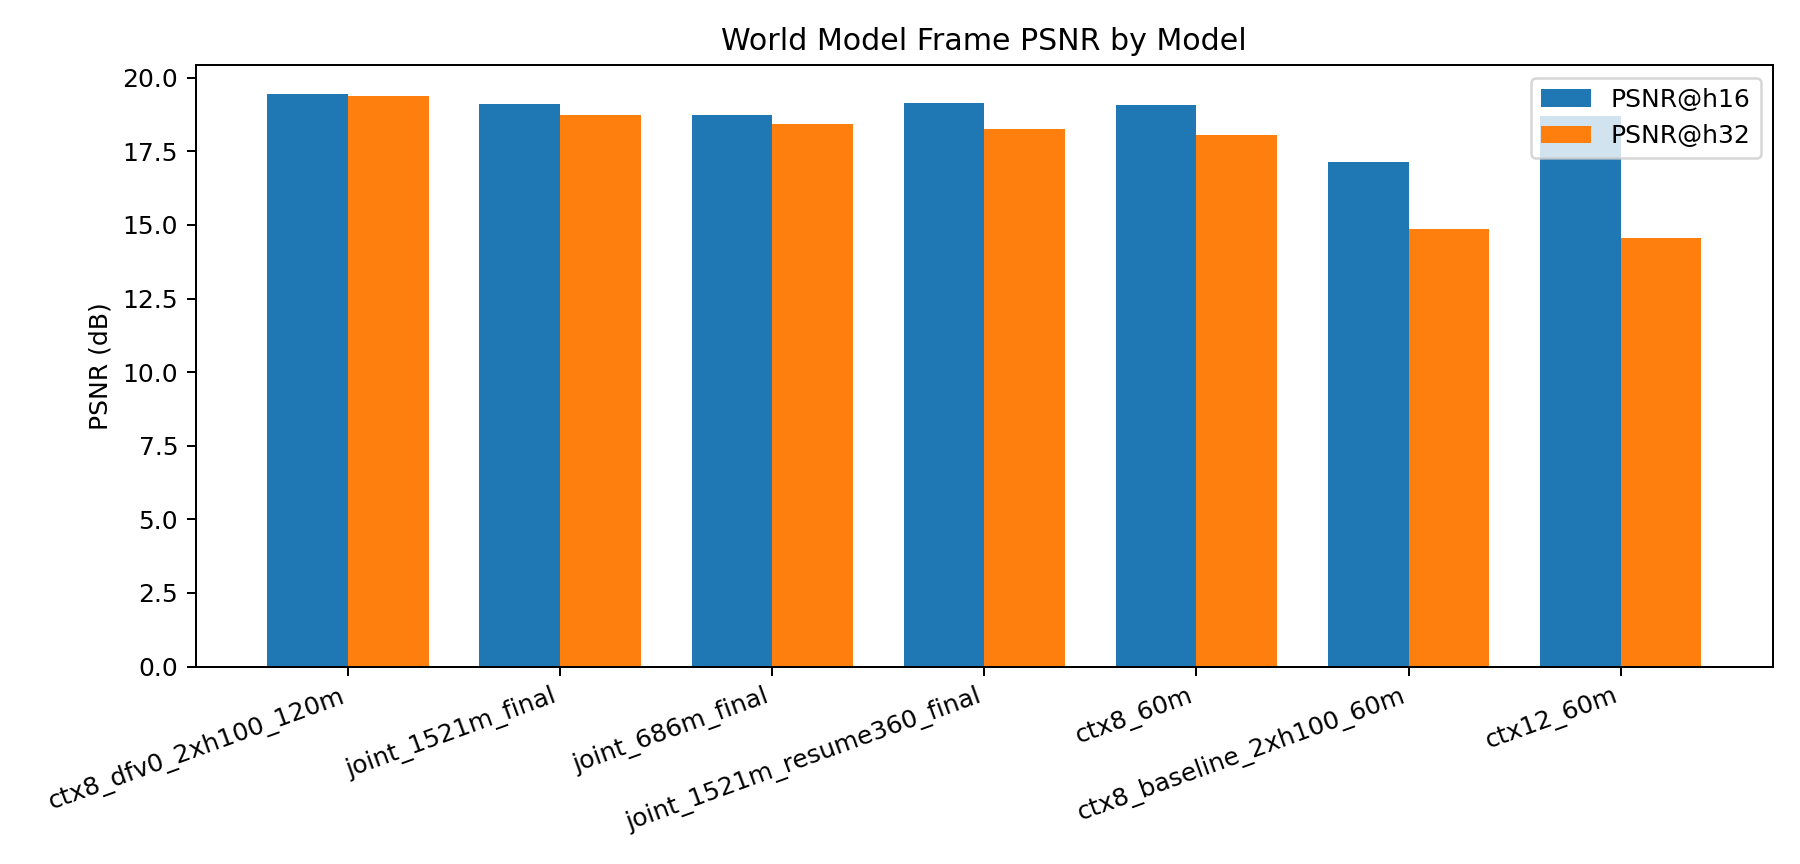
\includegraphics[width=\linewidth]{../../milestones_preview/charts/world_model_psnr_h16_h32.png}
\end{columns}
\vspace{0.3em}
\footnotesize
These charts summarize long-horizon behavior across milestone checkpoints.
\end{frame}

\begin{frame}{Hardships We Hit (And Why They Matter)}
\begin{itemize}
  \item \textbf{Physics artifacts:} color drift and occasional swallowing/merging.
  \item \textbf{Interactive inference:} high latency at low DDIM steps vs quality tradeoff.
  \item \textbf{Action loop:} early versions had weak action effect / unclear feedback, needed UI instrumentation.
  \item \textbf{Training ops:} run failures (NCCL watchdog abort, bad module path restart).
  \item \textbf{Evaluation rigor:} needed near-fair reruns and controls to avoid overclaiming.
\end{itemize}
\end{frame}

\begin{frame}{Limitations and Methodological Risks}
\begin{itemize}
  \item Near-fair is 60.0M vs 60.2M, not exactly equal sample count.
  \item Historical headline compare (60M vs 120M) mixes regime and budget effects.
  \item Eval currently uses independently sampled diffusion noise per model.
  \item Identity consistency remains the main unresolved artifact.
\end{itemize}
\vspace{0.4em}
\textbf{Mitigation plan}
\begin{itemize}
  \item deterministic/noise-shared paired eval for strict fairness
  \item color-consistency auxiliary loss with simulator masks
  \item collision-focused sampling with uniform-mix regularization
\end{itemize}
\end{frame}

\begin{frame}{Distillation Status (Teacher vs Student, Mar 4)}
\textbf{Eval run:} \texttt{rollout\_eval\_joint\_teacher555m\_vs\_distill573m\_20260304\_run01}
\vspace{0.3em}
\begin{table}
\centering
\begin{tabular}{lcccc}
\toprule
Model & MSE@16 & MSE@32 & PSNR@16 & PSNR@32 \\
\midrule
Teacher 1521M (ckpt 555M) & 0.662 & 0.957 & 19.04 & 18.09 \\
Student 573M (distill 30M) & 953.11 & 3185.85 & 11.06 & 8.70 \\
\bottomrule
\end{tabular}
\end{table}
\vspace{0.2em}
\textbf{Takeaway:} current student is much faster/smaller, but quality drops too much at long horizon.\\
Distillation is not yet ready to replace teacher for fidelity-critical demos.
\end{frame}

\begin{frame}{Next Steps}
\begin{enumerate}
  \item Strict fair ablation: matched 120M baseline vs matched 120M DF.
  \item Add color consistency loss on predicted \(x_0\).
  \item Stabilize distillation for faster interactive inference.
  \item Improve interactive UI: clearer action overlays + lower-latency generation.
\end{enumerate}
\vspace{0.5em}
\textbf{Current status:} DF already delivers a strong long-horizon robustness gain.
\end{frame}

\begin{frame}{Final Takeaways}
\begin{itemize}
  \item We validated the core hypothesis: DF improves long-horizon physics consistency.
  \item Wall bounce and collision coherence are now credible in many rollouts.
  \item Biggest remaining research gap is identity consistency (color/object persistence).
  \item This is now a solid base for a faster, more playable interactive world model.
\end{itemize}
\end{frame}

\begin{frame}{Supplementary Media}
For demo:
\begin{itemize}
  \item VAE reconstruction GIF:\\
  \texttt{milestones\_preview/final\_project\_media/vae\_latent\_compare\_ep0\_13s.gif}
  \item Latest rollout GIF:\\
  \texttt{milestones\_preview/final\_project\_media/latest\_resume555m\_clip\_002.gif}
\end{itemize}
\vspace{0.4em}
These are lightweight assets for fast playback in class.
\end{frame}

\end{document}
